\documentclass[tikz,border=10pt]{standalone}
\usepackage{amsmath,amssymb}
\usetikzlibrary{positioning,arrows.meta,calc}

\begin{document}
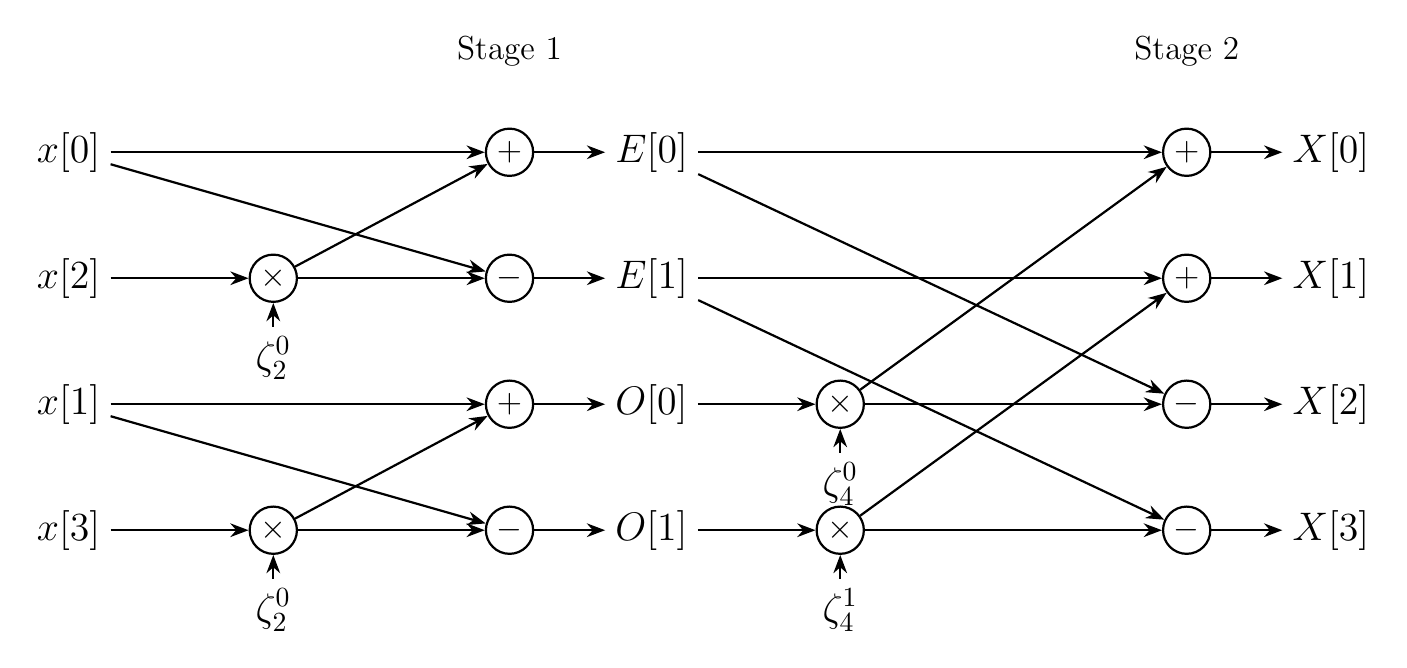
\begin{tikzpicture}[
  >=Stealth,
  thick,
  op/.style={circle, draw, minimum size=0.6cm, inner sep=0pt, font=\large}
]

% -----------------------
% Layout parameters
% -----------------------
\def\dy{1.6}

\def\xin{0}
\def\xmulA{2.6}
\def\xopA{5.6}
\def\xmid{8.6}
\def\xmulB{11.2}
\def\xopB{14.2}
\def\xout{17.2}

% y-levels (top to bottom)
\def\yA{ { 1.5*\dy} }   % line 0
\def\yB{ { 0.5*\dy} }   % line 1
\def\yC{ {-0.5*\dy} }   % line 2
\def\yD{ {-1.5*\dy} }   % line 3

% -----------------------
% Inputs
% -----------------------
\node (x0) at (\xin,\yA) {\Large $x[0]$};
\node (x2) at (\xin,\yB) {\Large $x[2]$};
\node (x1) at (\xin,\yC) {\Large $x[1]$};
\node (x3) at (\xin,\yD) {\Large $x[3]$};

% -----------------------
% Stage 1 (size-2 FFTs): (x0,x2)->(E0,E1) and (x1,x3)->(O0,O1)
% -----------------------

% Top butterfly: x0 (top), x2 (bottom)
\node[op] (tE) at (\xmulA,\yB) {$\times$};
\node[op] (pE) at (\xopA,\yA)  {$+$};
\node[op] (mE) at (\xopA,\yB)  {$-$};

\node[below=0.3cm of tE] (wE) {\Large $\zeta_2^{0}$};
\draw[->] (wE) -- (tE);

\draw[->] (x0) -- (pE);
\draw[->] (x0) -- (mE);

\draw[->] (x2) -- (tE);
\draw[->] (tE) -- (pE);
\draw[->] (tE) -- (mE);

\node[right=0.9cm of pE] (E0) {\Large $E[0]$};
\node[right=0.9cm of mE] (E1) {\Large $E[1]$};
\draw[->] (pE) -- (E0);
\draw[->] (mE) -- (E1);

% Bottom butterfly: x1 (top), x3 (bottom)
\node[op] (tO) at (\xmulA,\yD) {$\times$};
\node[op] (pO) at (\xopA,\yC)  {$+$};
\node[op] (mO) at (\xopA,\yD)  {$-$};

\node[below=0.3cm of tO] (wO) {\Large $\zeta_2^{0}$};
\draw[->] (wO) -- (tO);

\draw[->] (x1) -- (pO);
\draw[->] (x1) -- (mO);

\draw[->] (x3) -- (tO);
\draw[->] (tO) -- (pO);
\draw[->] (tO) -- (mO);

\node[right=0.9cm of pO] (O0) {\Large $O[0]$};
\node[right=0.9cm of mO] (O1) {\Large $O[1]$};
\draw[->] (pO) -- (O0);
\draw[->] (mO) -- (O1);

% -----------------------
% Stage 2 (final butterflies):
% (E0,O0)->(X0,X2) and (E1,O1)->(X1,X3)
% -----------------------

% Butterfly for (E0,O0) -> (X0,X2)
\begin{scope}[shift={(-1.4,0.)}]
  \node[op] (tX0) at (\xmulB,\yC) {$\times$};
\end{scope}
\node[op] (pX0) at (\xopB,\yA)  {$+$};
\node[op] (mX2) at (\xopB,\yC)  {$-$};

\node[below=0.3cm of tX0] (wX0) {\Large $\zeta_4^{0}$};
\draw[->] (wX0) -- (tX0);

\draw[->] (E0) -- (pX0);
\draw[->] (E0) -- (mX2);

\draw[->] (O0) -- (tX0);
\draw[->] (tX0) -- (pX0);
\draw[->] (tX0) -- (mX2);

\node[right=0.9cm of pX0] (X0) {\Large $X[0]$};
\node[right=0.9cm of mX2] (X2) {\Large $X[2]$};
\draw[->] (pX0) -- (X0);
\draw[->] (mX2) -- (X2);

\begin{scope}[shift={(-1.4,0.)}]

\node[op] (tX1) at (\xmulB,\yD) {$\times$};
\end{scope}
% Butterfly for (E1,O1) -> (X1,X3)
\node[op] (pX1) at (\xopB,\yB)  {$+$};
\node[op] (mX3) at (\xopB,\yD)  {$-$};

\node[below=0.3cm of tX1] (wX1) {\Large $\zeta_4^{1}$};
\draw[->] (wX1) -- (tX1);

\draw[->] (E1) -- (pX1);
\draw[->] (E1) -- (mX3);

\draw[->] (O1) -- (tX1);
\draw[->] (tX1) -- (pX1);
\draw[->] (tX1) -- (mX3);

\node[right=0.9cm of pX1] (X1) {\Large $X[1]$};
\node[right=0.9cm of mX3] (X3) {\Large $X[3]$};
\draw[->] (pX1) -- (X1);
\draw[->] (mX3) -- (X3);

% Optional: stage labels
\node[font=\large] at (\xopA, {2.3*\dy}) {Stage 1};
\node[font=\large] at (\xopB, {2.3*\dy}) {Stage 2};

\end{tikzpicture}
\end{document}
